\documentclass[12pt]{article}
\usepackage[margin=1in]{geometry}
\usepackage{amsmath}
\usepackage{graphicx}
\usepackage{setspace}
\usepackage{subcaption}
\usepackage{listings}
\usepackage[italicdiff]{physics}
\usepackage{natbib}
\usepackage{epstopdf}
\lstset{breaklines=true, tabsize = 3}

\author{Jonathan Bunton}
\title{Calculating Wavefunctions and Spectrum for an Electron in a Gaussian Well}
\date{\today}

\begin{document}
\maketitle
\onehalfspacing
\begin{abstract}
The calculation of wavefunctions in various potential proves incredibly useful in atomic models, where these wavefunctions represent electron orbitals behaving in various atomic potentials.  In this work, we consider an electron within a Gaussian potential function, defined by:
\begin{align}
\label{potentialeq}
V(x) &= -De^{-a\frac{x^2+y^2+z^2}{l^2}}
\end{align}
If we consider only the region bound by the interval $[-l,l]$ and assume this potential repeats, this problem loosely resembles an atomic lattice structure in three dimensions.  To solve this potential for the energy spectrum and wavefunctions, we build our solutions from the basis functions of the form:
\begin{align}
\label{basis}
f_n(x) &= \begin{cases}
\sqrt{\frac{L}{2}}\sin\left(\frac{n\pi x}{l}\right) & n > 0\\
\sqrt{\frac{L}{2}}\cos\left(\frac{n\pi x}{l}\right) & n \leq 0
\end{cases}
\end{align}
These basis functions form the solutions to the classic infinite square well problem in quantum mechanics, which form a complete orthonormal basis for our wavefunction to be constructed from.  Using a specified number of these basis functions (as infinite would be exact but computationally impossible), we construct our Hamiltonian matrix by calculating the expectation values of the potential and kinetic energy for each pair of terms.  These expectation values are found with integrals numerically evaluated using Boole's Rule. \cite{boolesrule}  We then use LAPACK to calculate the eigenvalues and eigenvectors, which correspond to the energies and appropriate weightings of each basis function. \cite{LAPACK} From the resulting eigenvectors, we can calculate values for the wavefunctions of interest in our region, and their corresponding eigenvalues indicate the energies. \cite{quantum}

The resulting spectra indicates that for the parameters $a = 4$, $l = 1\times 10^{-10}$, and $A = -2.179\times 10^{-17}$, we receive approximately 20 bound states, building our energy eigenvectors from only the five lowest energy basis functions. This simulation extracts ten of these states for four of the eight symmetry possibilities, with the other ten appearing as a result of the degeneracy and symmetry of the potential to rotation.  For bound states, the wavefunctions have negative energies, and also exhibit higher peaks in at least one dimension in the center of the well, as the probability of the electron being within the well is much higher for bound states.  With the energy eigenvalues, this code effectively builds the spectrum for the lowest energy states in this potential.
\end{abstract}

\section*{Results}
For visualization and conceptual understanding, this code is done in both the 1D case, and the 3D case.  Due to potential function's spherical symmetry, any of the results from the 1D case have analogs in 3D, making it interesting to discuss.  The parameters for the potential function used to create an "interesting" impact on the wavefunctions were $a = 4$, $l = 1\times 10^{-10}$, and $A = -2.179\times 10^{-17}$.
\subsection*{1-D Case}
In one dimension, the potential energy function reduces to a Gaussian in one coordinate:
\begin{align*}
V(x) &= De^{-a\frac{x^2}{l^2}},\quad\quad x\in [-l,l]
\end{align*}
The resulting function looks as shown in fig. \ref{potential}, with a large downward dip centered about the origin.  Due to its shape, we can expect the resulting wavefunctions to appear similar to those produced by the quantum harmonic oscillator potential $V(x) = x^2$, which makes since as the first term in the Taylor expansion of $e^x$ is also an $x^2$.  Based on the parameters used for our problem, we may see a varied number of bound states.  The deeper and wider the potential well is, (i.e. larger $D$ and $a$ terms in our function) the more bound states would be created for an electron within the potential. \cite{quantum}

\begin{figure}
\begin{center}
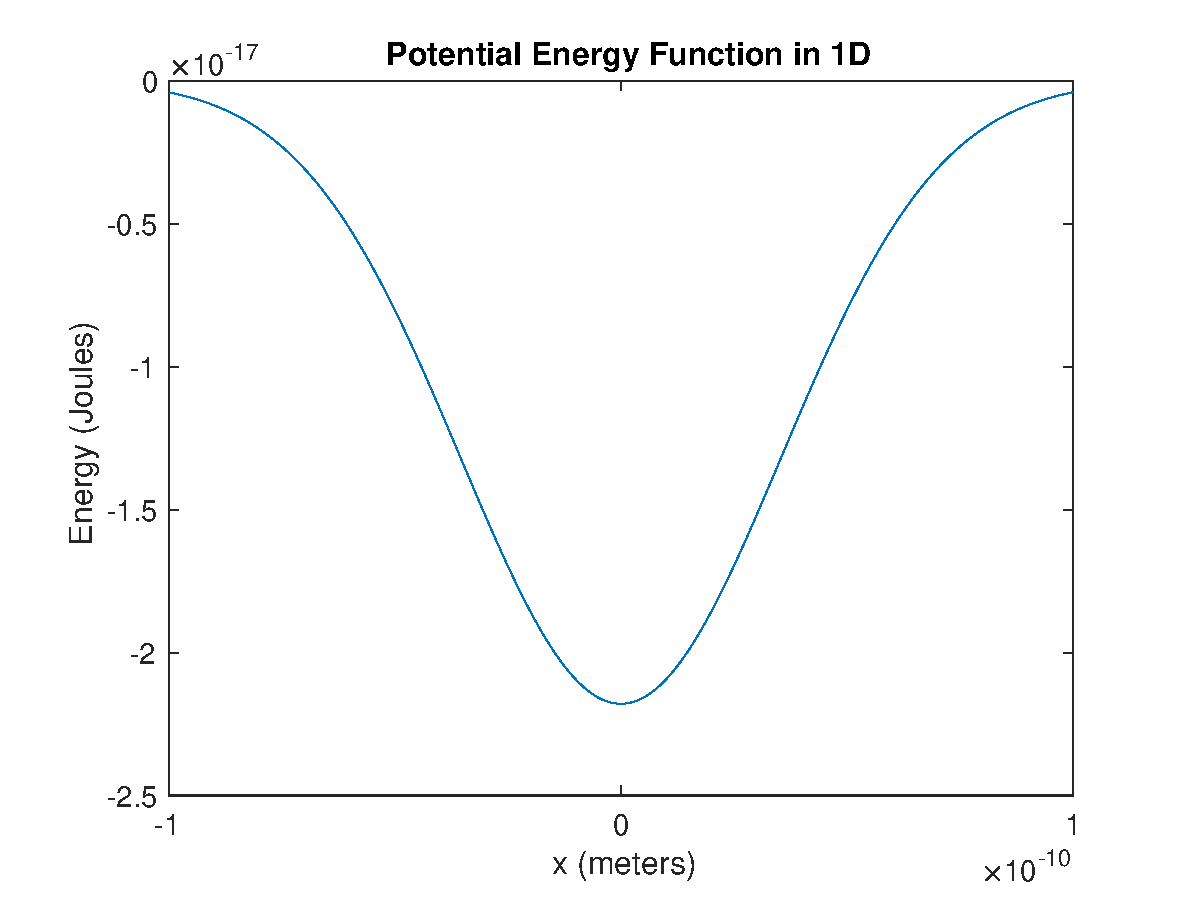
\includegraphics[width=0.7\textwidth]{./pics/potential.eps}
\end{center}
\caption{\label{potential} A plot of the potential energy function for the problem in question, in one dimension.  For the three dimensional case, this potential function exists across each dimension.}
\end{figure}

In the single dimensional case, there are only two basis function combinations: the sine terms in $f_n(x)$, and the cosine terms in $f_n(x)$.  This code splits the Hamiltonian for this system into two smaller Hamiltonians that represent those specific basis functions, and evaluates them individually.  This results in solutions in the form of effectively Fourier sine and cosine series, separately.  The lowest three wavefunctions in each basis are shown in figs. \ref{1dcosterms} and \ref{1dsinterms}.  The system emits three bound states given the potential parameters, which are characterized by the negative energies shown in the spectra, table \ref{1denergy}.  The wavefunctions found in the 1D case have analogs in three-dimensions, where various modes (values of $n$ in $f_n(x)$ as in eq. \ref{basis}) will contribute to the construction of a $f_{n,m,o}(x,y,z) = f_n(x)f_m(y)f_o(z)$.  These cause various 1D solutions to occur across each dimension in 3D space due to the symmetry in the problem.

\begin{figure}
\begin{center}
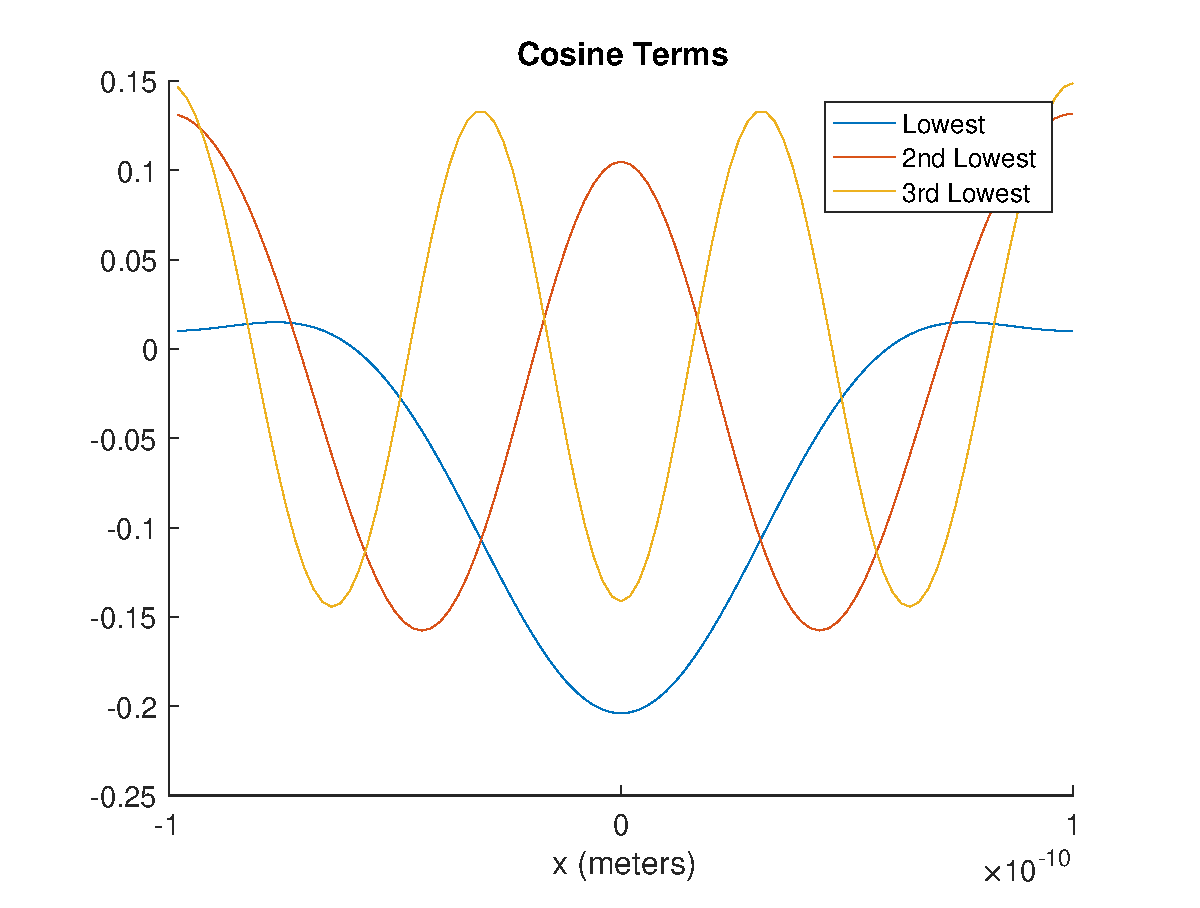
\includegraphics[width=0.6\textwidth]{./pics/1dcosterms.eps}
\end{center}
\caption{\label{1dcosterms}A plot of the three lowest energy cosine basis wavefunctions in one dimension.  The two lowest energy wavefunctions (pictured in blue and orange) are bound states, visualized by the maximums and minimums occurring in the center of the potential well, creating a higher probability of the electron being found within the potential well. These bound states are easily identified by negative energies, which are approximately -5.01$\times 10^{-17}$ J and -1.62$\times 10^{-19}$ J.}
\end{figure}

\begin{figure}
\begin{center}
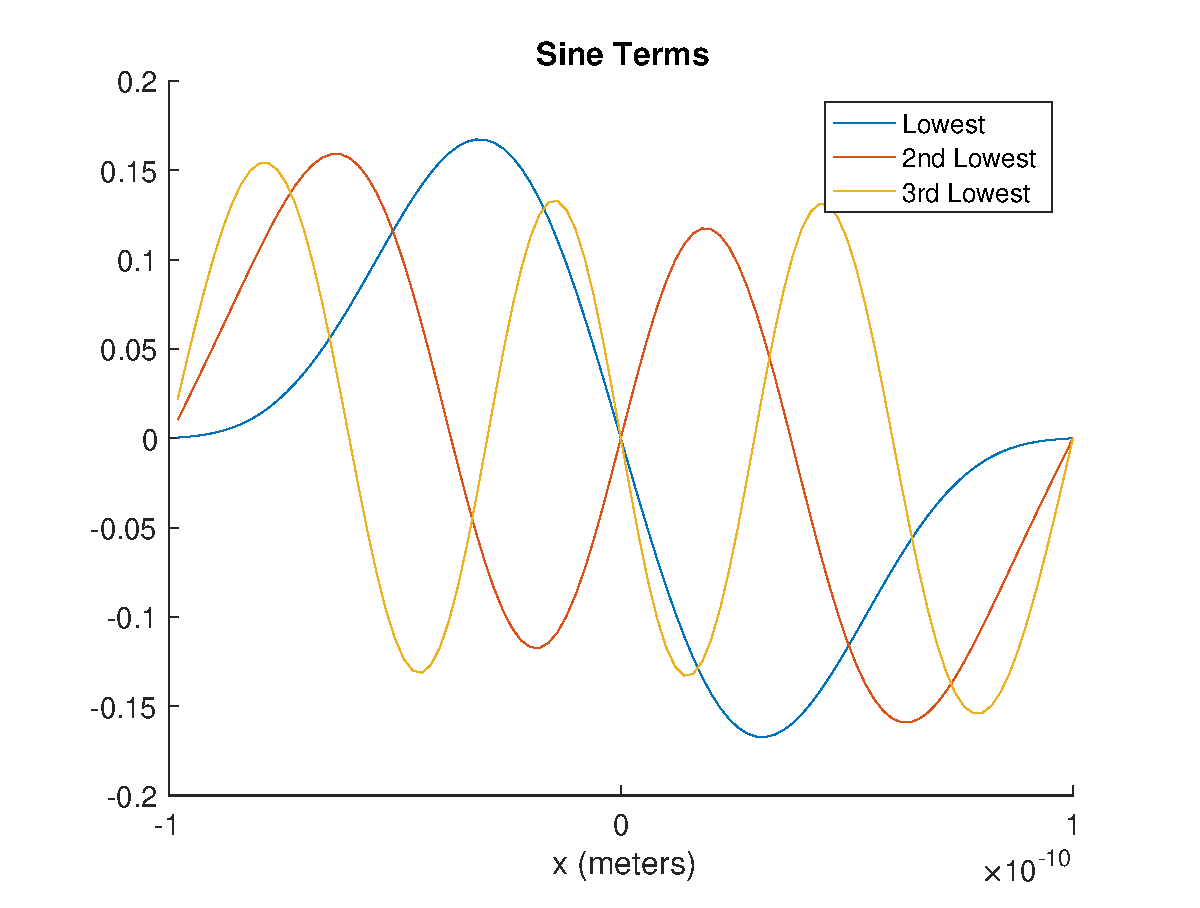
\includegraphics[width=0.6\textwidth]{./pics/1dsinterms.eps}
\end{center}
\caption{\label{1dsinterms}A plot of the first three lowest energy sine basis wavefunctions in one dimension.  Only the lowest energy term (pictured in blue) is a bound state, visualized by the wavefunction's maximums and minimums occurring in the center of the potential well, creating the highest probability of the electron's location being within the well.  In addition, this bound state has a negative energy of approximately -1.74$\times 10^{-17}$ J.}
\end{figure}

\begin{table}
\begin{center}
\begin{tabular}{|c|c|c|}
\hline
Energy Level & Energy (Joules) & Symmetry (sin/cos) \\
\hline
1 & -5.01$\times 10^{-17}$ & $cos$\\
2 & -1.74$\times 10^{-17}$& $sin$ \\
3 & -1.62$\times 10^{-19}$& $cos$\\
4 & 6.97$\times 10^{-18}$& $sin$\\
5 & 3.02$\times 10^{-17}$ & $cos$ \\
6 &3.60$\times 10^{-17}$ & $sin$ \\
7 & 7.78$\times 10^{-17}$ & $sin$\\
8 & 8.98$\times 10^{-17}$&  $cos$\\
9 & 1.33$\times 10^{-16}$& $sin$ \\
10 & 1.74$\times 10^{-16}$& $cos$ \\
\hline
\end{tabular}
\caption{\label{1denergy} A table containing the values for the lowest 10 energy eigenfunctions for the 1D Gaussian potential.  The negative energy terms correspond to bound states within the potential.}
\end{center}
\end{table}

\subsection*{3D Case}
The true problem in question is the three-dimensional case, where the potential takes the form laid out in eq. \ref{potentialeq}.  This results in four-dimensional data, with our wavefunctions being of form $f_{nmo}(x,y,z)$.  As in the 1D case we expect our wavefunctions to look reminiscent of the quantum harmonic oscillator solutions, however, these will take varying $n$ values for each $f_n$ in each dimension, causing the axes to take the form of differing solutions to the 1D equation laid out above.

In the 1D case we considered only the two basis functions, however, for three dimensions, each of the three dimensions can take either sine or cosine bases functions from $f_n$, meaning if we attempted to split the Hamiltonian into individual portions, we would need to analyze $2^3 = 8$ basis combination Hamiltonians.  Because of the symmetry inherent in the potential, we instead only consider the combinations which produce wavefunctions that are unique under rotations, namely the combinations $sin/sin/sin$, $sin/sin/cos$, $sin/cos/cos$, and $cos/cos/cos$.  Because of the nature of the symmetry, there is some inherent degeneracy in the energy spectrum.  This is shown in the resulting energy spectrum for the lowest 20 eigenstates, table \ref{3denergies}.

\begin{table}
\begin{center}
\begin{tabular}{|c|c|c|}
\hline
Energy State & Energy (Joules) & Symmetry (x-trig/y-trig/z-trig)\\
\hline
1 & -7.15$\times 10^{-31}$ & $sin/cos/cos$ \\
2 & -3.75$\times 10^{-31}$ & $sin/cos/cos$ \\
3 & -3.185$\times 10^{-31}$& $sin/cos/cos$ \\
4 & -1.74$\times 10^{-31} $ & $sin/cos/cos$ \\
5 & -1.44$\times 10^{-31}$ & $sin/cos/cos$ \\
6 & 1.76$\times 10^{-31}$ & $cos/cos/cos$ \\
7 & 1.20$\times 10^{-31}$ & $cos/cos/cos$ \\
8 & 1.20$\times 10^{-31}$ & $cos/cos/cos$ \\
9 & 1.20$\times 10^{-31}$ & $cos/cos/cos$ \\
10 & 2.41$\times 10^{-17}$ & $cos/cos/cos$ \\
11 & 2.41$\times 10^{-17}$ & $sin/sin/cos$ \\
12 & 3.61$\times 10^{-17}$ & $sin/sin/cos$ \\
13 & 3.61$\times 10^{-17}$ & $sin/sin/sin$ \\
14 & 6.02$\times 10^{-17}$ & $sin/sin/cos$ \\
15 & 6.02$\times 10^{-17}$ & $sin/sin/cos$ \\
16 & 7.23$\times 10^{-17}$ & $sin/sin/cos$ \\
17 & 7.23$\times 10^{-17}$ & $sin/sin/sin$ \\
18 & 7.23$\times 10^{-17}$ & $sin/sin/sin$ \\
19 & 7.23$\times 10^{-17}$ & $sin/sin/sin$ \\
20 & 1.08$\times 10^{-16}$ & $sin/sin/sin$ \\
\hline
\end{tabular}
\end{center}
\caption{\label{3denergies}A table describing the energies of the 20 lowest energy wavefunctions with unique (under rotation) wavefunctions.  Even among these 20 wavefunctions there is clear degeneracy.  In addition, negative energy terms indicate bound states, leading to the conclusion that there are five bound states with unique symmetries for these potential parameters.}
\end{table}

To properly visualize the 4-dimensional data, we take 3-dimensional slices of the data to plot.  The lowest energy wavefunction is shown with each $x$, $y$, and $z$ held constant at 0 separately in figs. \ref{lowestx0}, \ref{lowesty0}, and \ref{lowestz0}.  Bound states exhibit wavefunction deviation toward minimums and maximums in the regions at the center of the Gaussian potential (point $(0,0,0)$), whereas free states show no change as they pass over the potential well.  In addition, these solutions are periodic, which means we can picture them repeating over all three dimensions to represent an electron in a full 3D lattice.  Bound states would indicate that in at least one dimension, the electron is effectively ``trapped" in the wells, and will not be shared with the other atoms in the lattice.  For free states, the electrons have enough energy to be shared with other atoms within the lattice.

\begin{figure}
\begin{center}
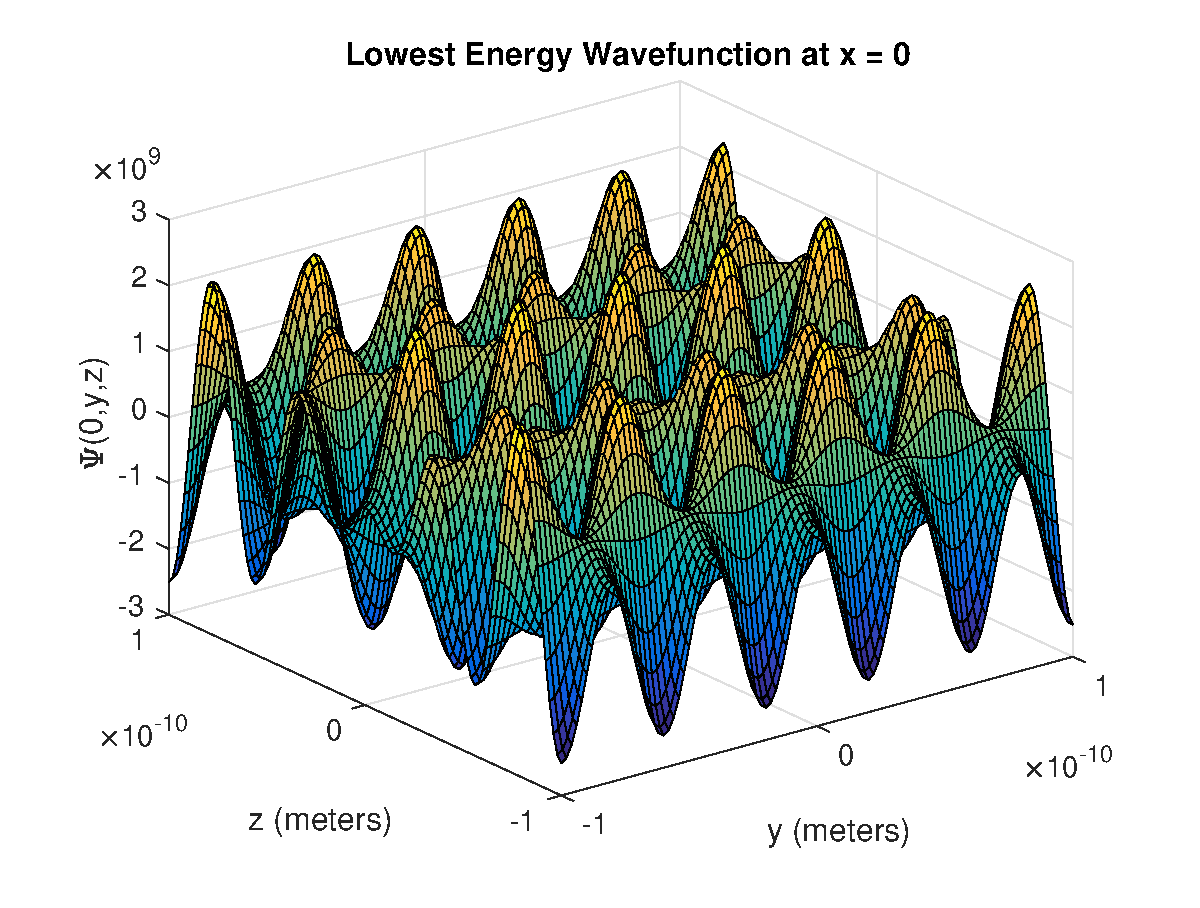
\includegraphics[width=0.7\textwidth]{./pics/lowest3dx0.eps}
\end{center}
\caption{\label{lowestx0}The lowest-energy wavefunction plotted with $x=0$.  The function shows no variation as it nears the center of the Gaussian potential.}
\end{figure}

\begin{figure}
\begin{center}
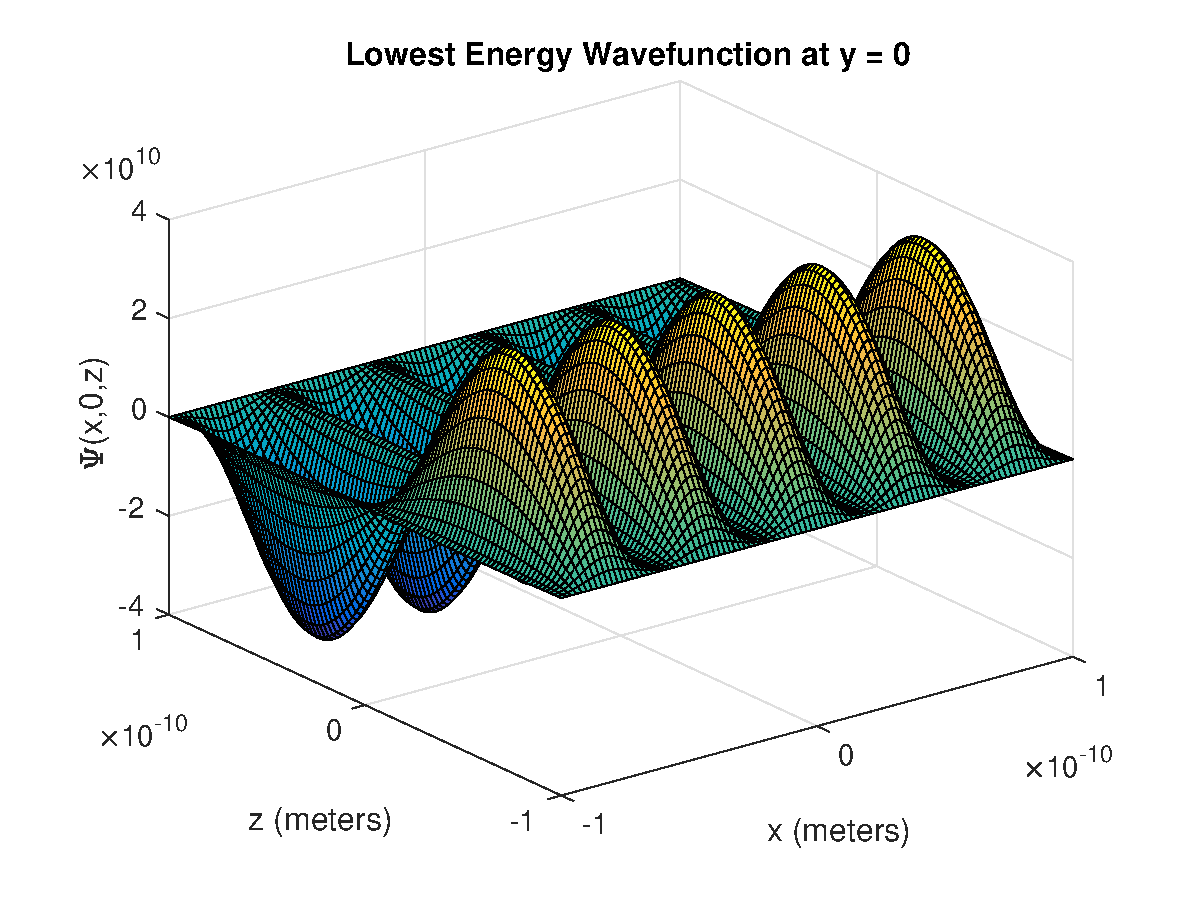
\includegraphics[width=0.7\textwidth]{./pics/lowest3dy0.eps}
\end{center}
\caption{\label{lowesty0}The lowest-energy wavefunction plotted with $y=0$.  The function again shows no variation near the center of the Gaussian potential.}
\end{figure}

\begin{figure}
\begin{center}
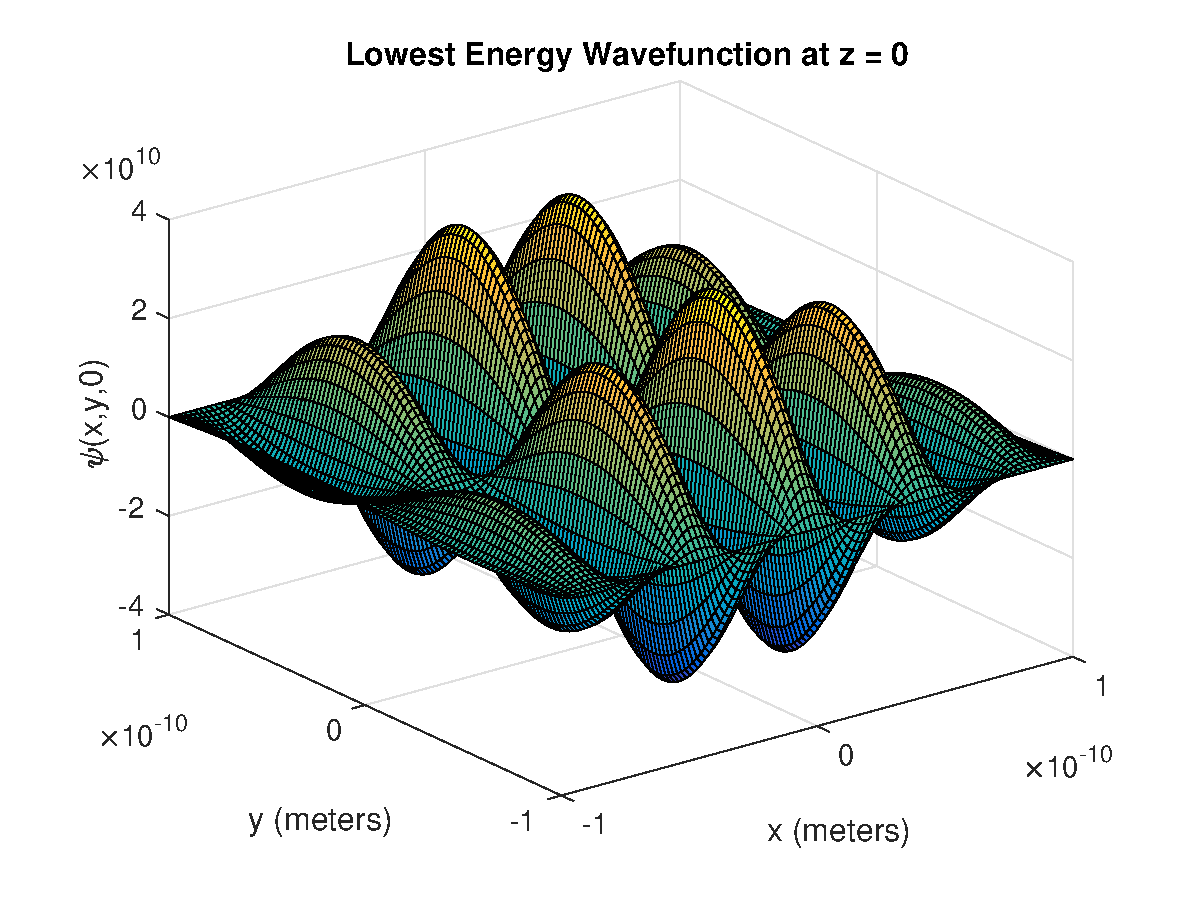
\includegraphics[width=0.7\textwidth]{./pics/lowest3dz0.eps}
\end{center}
\caption{\label{lowestz0}The lowest-energy wavefunction plotted with $z=0$.  The maximum in the wavefunction toward the center of the Gaussian potential, which points to the bound-state nature of this energy state.}
\end{figure}

To illustrate the difference between bound and free states, the plots of the 19\textsuperscript{th} wavefunction from table \ref{3denergies} are shown in figs. \ref{19x0}, \ref{19y0}, and \ref{19z0}.  In contrast, these wavefunctions display no minimums or maximums around the center of the Gaussian potential, which indicates the electron is ``less likely" to be found in this location.

\begin{figure}
\begin{center}
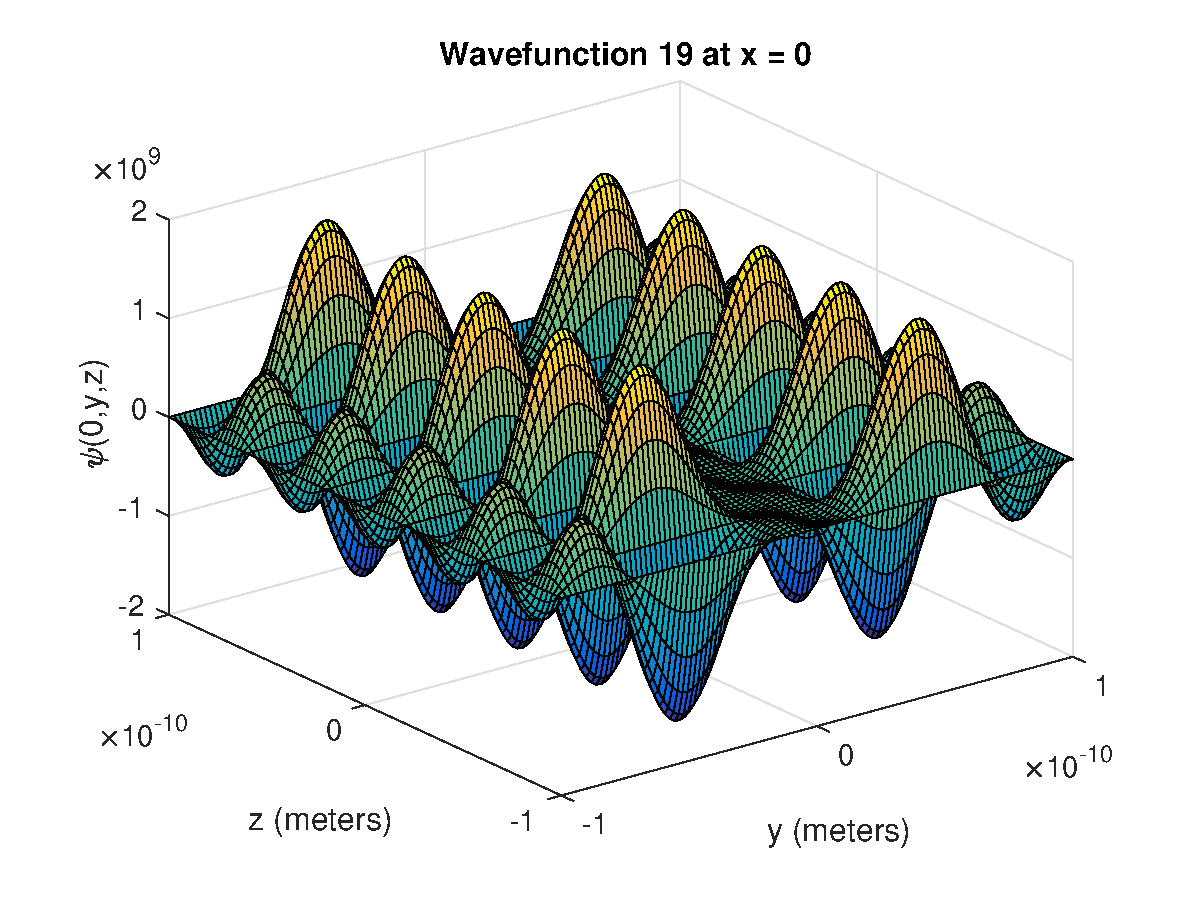
\includegraphics[width=0.7\textwidth]{./pics/wfn19x0.eps}
\end{center}
\caption{\label{19x0}Wavefunction 19 from table \ref{3denergies}, plotted at $x=0$.  This state is a free state, with positive energy, which is clear from the lack of wavefunction minimum or maxima at the center of the Gaussian well.}
\end{figure}

\begin{figure}
\begin{center}
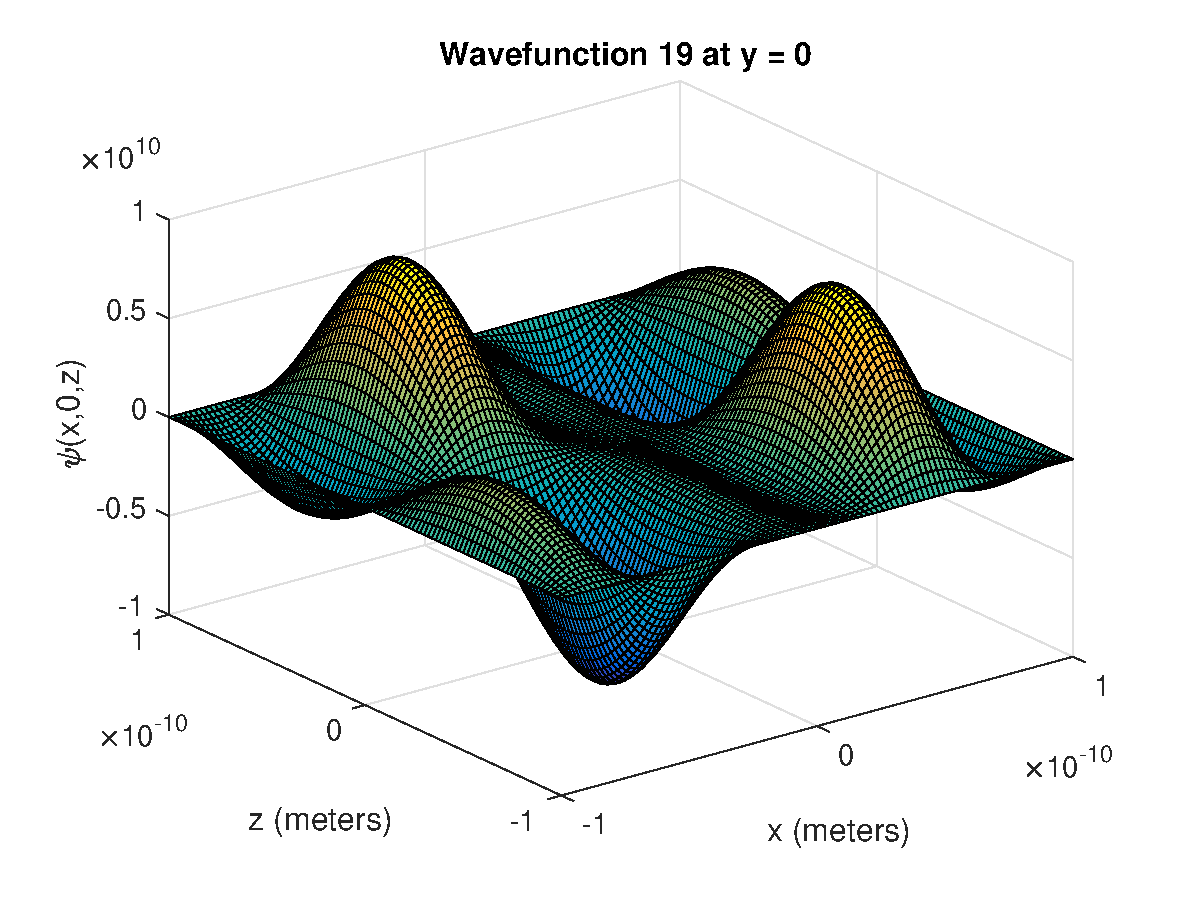
\includegraphics[width=0.7\textwidth]{./pics/wfn19y0.eps}
\end{center}
\caption{\label{19y0}Wavefunction 19 from table \ref{3denergies}, plotted at $y=0$.  This state is a free state, with positive energy, which is clear from the lack of variation in the wavefunction at the center of the Gaussian well.}
\end{figure}

\begin{figure}
\begin{center}
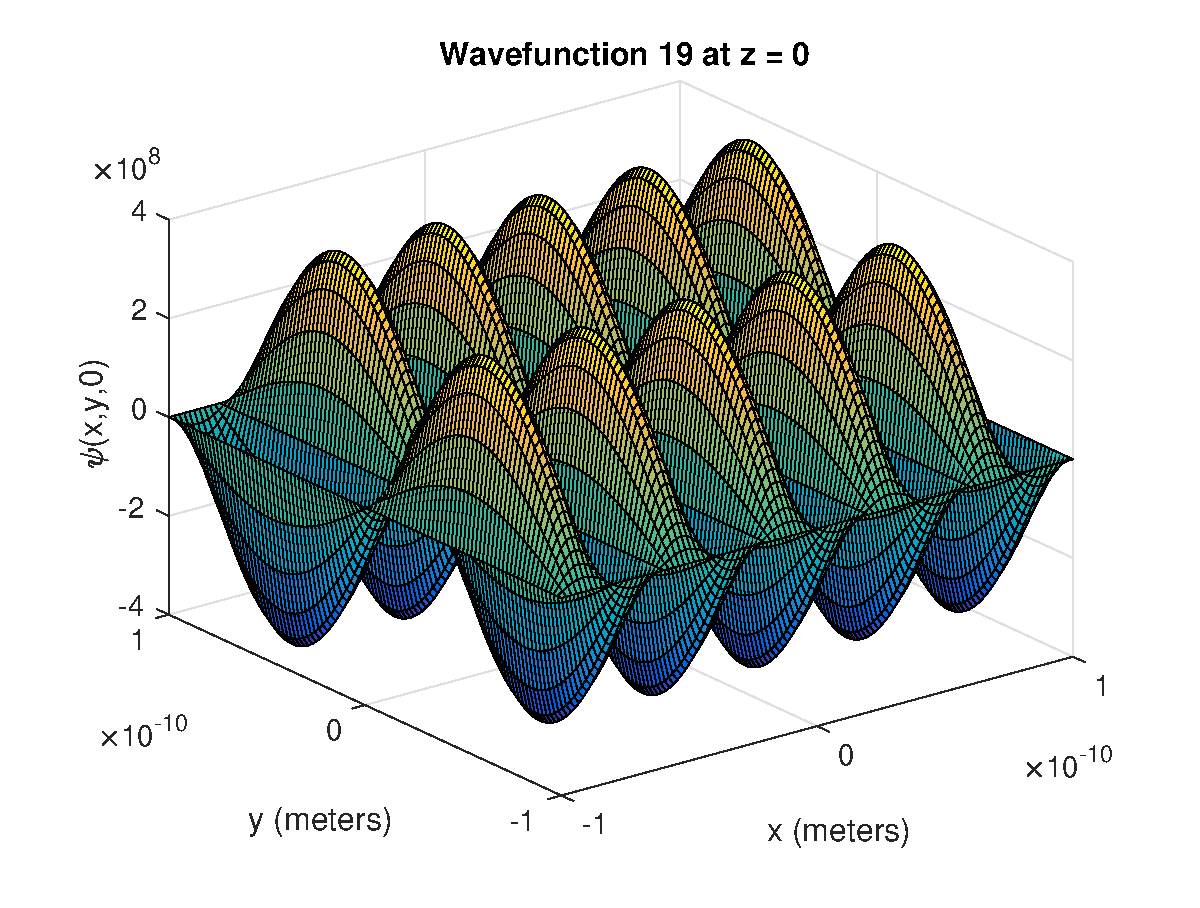
\includegraphics[width=0.7\textwidth]{./pics/wfn19z0.eps}
\end{center}
\caption{\label{19z0}Wavefunction 19 from table \ref{3denergies}, plotted at $z=0$.  This state is a free state, with positive energy, which is clear from the lack of variation in the wavefunction at the center of the Gaussian well.}
\end{figure}

There are ultimately four more combinations of basis trig functions available in each dimension, where the sine and cosine terms are permuted through the $x$, $y$, and $z$ axes, but these will yield identical shapes to those in the initial four symmetries in this paper, transformed only by a rotation.  These will also show degeneracy in the energies accordingly.  On this basis, we need only examine the first four combinations of basis functions to understand the behavior of the remaining permutations.

\subsection*{Discussion}
The resulting energy spectrum shows that for the given parameter values for a Gaussian potential in three dimensions, $a = 4$, $l = 1\times 10^{-10}$, and $A = -2.179\times 10^{-17}$, there are ten bound states.  Building these resulting wavefunctions from a series of only five terms yields the energy spectrum in three dimensions shown in table \ref{3denergies}.  Looking at the solutions to the one-dimensional case shows clear analogies to the three dimensional functions, where the eigenfunctions make up the functions along each axis.  The three-dimensional eigenvalues show some degeneracy, where multiple eigenfunctions can yield identical energies due to ability to assign each basis function's energy to different axes without changing its value.

Bound wavefunctions exhibit maximums and minimums around the center of the Gaussian well, indicating a higher probability of the electron's position being within the well.  In contrast, free states show no change over the well, or no minimums and maximums at the center.  In the case of an atomic lattice, bound states indicate the electrons have insufficient energy to be shared between the atoms.  Conversely, free states indicate the electron may be free to move between the various atoms that comprise the lattice.

Using Boole's Rule to calculate the inner products required to construct the Hamiltonian matrices and LAPACK to calculate the eigenvectors and values of said matrices, we have accurately approximated the energy spectrum for an electron in our specified Gaussian potential well, and also retrieved approximations for the wavefunctions in the lowest twenty eigenstates.
\pagebreak
\section*{Acknowledgements}
I would like to thank Dr. Justin Oelgoetz for assistance formulating the simulation code, and for providing insightful explanations and troubleshooting along the way.

All graphs and plots made in this paper were produced using MATLAB computational software.
\newpage
\bibliographystyle{plain}
\bibliography{quantum}
\newpage
\section*{Appendix}
Attached is the source code for this project, written in Fortran.
\subsection*{Main}
\lstinputlisting[language=Fortran]{../quantum.f90}
\subsection*{Integration Module}
\lstinputlisting[language=Fortran]{../integrateme.f90}
\subsection*{Constants Module}
\lstinputlisting[language=Fortran]{../constants.f90}
\subsection*{MATLAB Plotting Script}
Code can be run while MATLAB is in the directory containing result files and will create a .gif file of positions, total energy and momentum plots, an initial velocity sampling histogram, average displacement magnitude vs. time, and initial and final scatter plots of position and save them to the directory.
\lstinputlisting[language=Octave]{../threedeeplots.m}
\end{document}